In this chapter, various models describing the mechanism of proton-induced spallation reactions will be discussed. According to Serber \cite{Serber}, such a reaction can proceed in two steps. The first stage is a cascade of binary collisions which occur in a few fm/c and mainly consisted of the emission of nucleons, pions, and light complex particles leaving the exciting remnant of the target nucleus in the equilibrium.  The second stage of the reaction consists of de-excitation of this remnant nucleus by various processes like evaporation, multi-fragmentation, asymmetric fission and symmetric fission which produces usually the "light charge particle-LCP", Intermediate Mass Fragments(IMF) and heavy residue. There few models available which assumed three steps of the reaction. They assume one more intermediate state between cascade and evaporation state. They called this state a pre-equilibrium state. In the next sections, various models of the first and second stage of two-step reactions will be described.
\section{Models of the first stage reactions}
Various first stage models were developed during several last decades like INCL \cite{INCLCugnon1981,INCLboudard2002intranuclear,INCLboudard2004new,INCLboudard2013new,INCLMancusi2014}, GiBUU\cite{GiBUUBuss2012}, UrQMD\cite{UrQMDBASS1998,UrQMDBleicher1999}, JAM\cite{JAM_NARA1999}, INC by Bertini\cite{Bertini1963,Bertini1969}, CEM\cite{CEM_GUDIMA1983}, and ISABEL\cite{Isabel_Yariv1979,Isabel_Yariv1981}, etc. Here the most popular of them will be discussed.

\subsection{Intranuclear cascade models - INC}\label{INC}
The models which assume, that the interactions of high-energy particles with the nucleus can be represented by free nucleon-nucleon and nucleon-pion collisions inside the nucleus are called intranuclear cascade models. The 1st code of INC-type has been created by Bertini in 1963\cite{Bertini1963,Bertini1969}. Later, the conception was used also in other codes, e.g. by Yariv in his ISABEL code\cite{Isabel_Yariv1979,Isabel_Yariv1981}. 
In the 80's and 90's, the several versions of INC model were developed by Cugnon et al.\cite{INCLCugnon1981,INCLboudard2002intranuclear,INCLboudard2004new,INCLboudard2013new}(The newest version is INCL++5.6 \cite{INCLMancusi2014}).
\begin{figure}
	\centering
	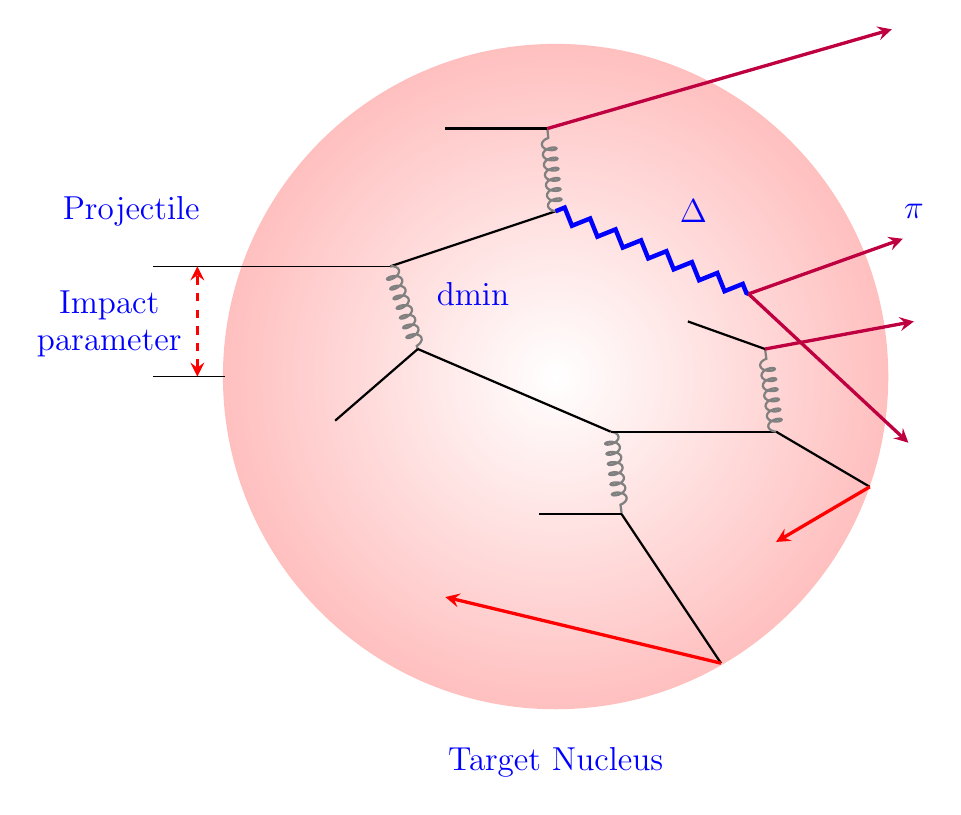
\begin{tikzpicture}[scale=0.7]
		
		\node[circle,outer color=pink!100!black,inner color=white,minimum width=8.45cm] (radial) at (0,0) {};
		\proton{-7.7,2};
		\proton{-2.3,4.5}
		\neutron{-4.3,-1};
		\proton{2.1,1.1}
		\pion{6.5,2.5}
		\proton{-0.6,-2.5};
		%\draw[ultra thick] (0,0) circle (6 cm);
		\draw[blue](2.5,3) node {\large $\Delta$};
		\draw[blue](-1.5,1.5) node {\large dmin};
		\draw[blue](6.5,3) node {\large $\pi$};
		\draw[blue](-7.7,3) node {\large Projectile};
		\draw[blue](-8.1,1.3) node {\large Impact};
		\draw[blue](-8.1,0.6) node {\large parameter};
		\draw[blue](0,-7) node {\large Target Nucleus};
		\draw [-](-7.3,2) --(-3,2);
		\draw [<->,>=stealth,very thick,color=red,dashed](-6.5,0) --(-6.5,2);
		\draw [-](-7.3,0) --(-6,0);
		\draw [-,thick](-3,2) --(0,3);
		\draw [color=gray,thick,decorate,decoration={coil,segment length=1.3mm, amplitude=0.9mm}](0,3) --(-0.15,4.5);
		\draw [-,thick](-2,4.5) --(-0.15,4.5);
		\draw [->,>=stealth,very thick,color=purple](-0.15,4.5) --(6.1,6.3);
		\draw [decorate,decoration={zigzag},ultra thick,color=blue](0,3) --(3.5,1.5);
		\draw [->,>=stealth,very thick,color=purple](3.5,1.5) --(6.3,2.5);
		\draw [->,>=stealth,very thick,color=purple](3.5,1.5) --(6.4,-1.2);
		\draw [color=gray,thick,decorate,decoration={coil,segment length=1.3mm, amplitude=0.9mm}](-3,2) --(-2.5,0.5);
		\draw [-,thick](-4,-0.8) --(-2.5,0.5); 
		\draw [-,thick](-2.5,0.5) --(1,-1);
		\draw [color=gray,thick,decorate,decoration={coil,segment length=1.3mm, amplitude=0.9mm}](1,-1) --(1.2,-2.5);
		\draw [-,thick](-0.3,-2.5) --(1.2,-2.5);
		\draw [-,thick](1.2,-2.5) --(3,-5.2);
		\draw [->,>=stealth,very thick,color=red](3,-5.2) --(-2,-4);
		\draw [-,thick](1,-1) --(4,-1);
		\draw [color=gray,thick,decorate,decoration={coil,segment length=1.3mm, amplitude=0.9mm}](4,-1) --(3.8,0.5);
		\draw [-,thick](2.4,1) --(3.8,0.5);
		\draw [->,>=stealth,very thick,color=purple](3.8,0.5) --(6.5,1);
		\draw [-,thick](4,-1) --(5.7,-2);
		\draw [->,>=stealth,very thick,color=red](5.7,-2) --(4,-3);
	\end{tikzpicture}
	\caption{Schematic view on INCL model main features}
	\label{INCLsch}
\end{figure}
In this thesis, INCL++ was used for the validation of different proton-induced reactions. Since the INC models are very similar to each other only the most advanced of them, i.e. INCL4.6 (INCL++) is described here. Please note that INCL4.6 \cite{INCLboudard2013new} is not identical with INCL++ \cite{INCLMancusi2014}. Text from ref\cite{INCLMancusi2014} :"The physics of the new code is substantially equivalent to the reference FORTRAN77 version INCL4.6 for nucleon- and pion-induced reactions; the few minor differences will be highlighted in Sec. IIA". The  INCL++ is also included in Geant4\cite{Geant_AGOSTINELLI2003250} code which is a well-accepted simulation code for various applications in high energy, space and radiation, as well as in medical fields. In figure \ref{INCLsch} the main features of INCL are represented.

\subsubsection{Assumptions of INCL\cite{INCLboudard2002intranuclear} model}\label{FeaOFINCL}

\begin{enumerate}[label=(\roman*)] 
	
	\item Nucleons move inside the nucleus along straight trajectories until two of them collide or until one nucleon reaches the nucleus surface, where it can be transmitted or reflected (shown in figure \ref{INCLsch}).
	\item The collision takes place when the distance between two nucleons is smaller than $d_{min}$ which is given by:
	\begin{equation}
		d_{min}\leq\sqrt{\sigma_{tot}/\pi}
	\end{equation}
	where $\sigma_{tot}$ is the total nucleon-nucleon cross section
	\item The initial momentum and position are stochastically selected from the Fermi sphere described in next section.
	\item Relativistic kinematics is used in this model.
	\item The nucleons are divided into participants and spectators. The nucleons which are in cascade collision state are known as participants and those still not collided with participant are known as spectators.
\end{enumerate}


\subsubsection{Target Nucleus construction in INCL}\label{TargetNucleus}
The spatial distribution $\rho (r)$ of nucleons inside the target nucleus is prepared according to a Saxon-Woods formula (for detail see \cite{INCLboudard2013new})\\
\begin{equation}
	\rho (r)= \begin{cases} \frac{\rho_{0}}{1+\exp(\frac{r-r_{0}}{a})} &  r<R_{max}\\ 
		0 &  r> R_{max} \end{cases} 
\end{equation}
where $R_{max}=r_{int} + R_{0} + 8a$ and $r_{int}=(\sigma_{NN}^{tot}/\pi)^\frac{1}{2}$, 
The R$_{0}$ and $a$ values are taken from electron scattering measurements and parametrized for Al to U as below, where $A_T$ is the mass number of the target nucleus

\begin{align}
	R_{0} &=(2.7545*10^{-4}A_{T}+1.063)A_{T}^{1/3}\\
	a &=0.510 + 1.63 *10^{-4}A_{T}
\end{align}
The initial position and momentum of any target nucleon are generated as follows. First momentum P is taken randomly from a sphere of radius P$_{F}$. Then  R(p) corresponding to  momentum P is calculated by equation \ref{prp}. After that position r is randomly selected from the sphere of radius R(p).
\begin{align}
	\left(\frac{P}{P_{F}}\right)^{3}&=-\frac{4\pi}{3A_{T}}\int_{0}^{R(p)}\frac{d\rho(r)}{dr}r^{3}dr,\label{prp}
\end{align}
\subsubsection{Potential}
There are mainly three types of potential used in the model as it is described below.

a.) Isospin and energy-dependent potential well\cite{INCLaoust2004effects} : for the nucleons was used in  INCL\cite{INCLboudard2013new}. The potential depths which can be felt by nucleons are different for proton and neutron. The potential also varies with the energy of nucleons. Approximately the potential energy is decreasing with the energy of the nucleons.\\
\textit{Isospin dependence}: The neutrons and protons feel different respective potential depths $V_0^i$ for $i=n,p$. Let $k_F^n$ and $k_F^p$ are their Fermi momenta then respective kinetic energy can be calculated by:
\begin{equation}\label{FKE}
	T_F^{i}=\frac{(\hbar k_F^i)^2}{2M}
\end{equation}
Where M is the mass of the nucleon (same for neutron and proton)
From Koopman's theorem \cite{KOOPMANS1934104}, the total Fermi energy for proton and neutron  equals the separation energy: 
\begin{equation}
	T_F^{i}-V_0^i=-S_i
\end{equation}
The separation energy $S_i$ are taken from experiment\cite{WAPSTRA198555}. Then the depth of potential can be calculated by the above formula.\\ 
\textit{Energy dependence}: The following nucleon potential was adopted for energy dependence:
\begin{equation}\label{Epoten}
	V_{0}^{i}(E)= \begin{cases} V_{0}^{i}-\alpha\left(E-E_F^{i}\right) &  E<E_{0}\\ 
		0 &  E> E_{0} \end{cases} 
\end{equation}
where energy E of nucleon can be calculated by:
\begin{align}
	E=\frac{\hbar^2k^2}{2M}+V_{0}^{i}(E) \label{energy}
\end{align}
and the Fermi energy of nucleon $E_F^i$ is also defined by the same expression replacing $k=k_F^i$. The $E_0$ is the energy where $V_0^i =\alpha(E-E_F^i)$. The value of both parameters $\alpha_p$  and $\alpha_n$ is equal 0.23.
\\
\textit{Smoother energy dependence:} An option of smoother energy dependence is also introduced
\begin{equation}
	V_{0}^{i}(E)= V_{0}^{i}\exp\left(-\beta_i\left(E-E_F^i\right)\right)
\end{equation}
where $\beta=0.00681$ \cite{INCLboudard2004new} .The energy dependence for $\Delta$ particles are neglected.
\par
b.) Average potential for pions\cite{INCL_Aou_2006}:  An average isospin dependent potential well of the Lane type \cite{Lane1962PhysRevLett} is introduced for pions. For $\pi$ simple phenomenology potential form was used which is given by:
\begin{align}
	V\left(r,\tau_3\right)&=V_t(\tau_3)=V_N(\tau_3)+\overline{V}_C,& \text{ for } r<R_c \label{piopot}\\ 
	V\left(r,\tau_3\right)&=V_C(r)=\frac{Z_T\tau_3e^2}{r},& \text{ for } r>R_c 			\label{colpotpi}
\end{align}
where $\tau_3$ is the third component of $\pi$ isospin and Z$_T$ is target charge number. For the condition $r>R_c$  the potential reduces to Coulomb potential which is given by \eqref{colpotpi}. When r  is smaller than R$_c$ the Coulomb potential is fixed at constant value and the nuclear potential V$_N$ has similar form as of lane type potential given by:
\begin{equation}
	V_N(\tau_3)=V_N^{0}+V_N^{1}\tau_3\xi 
\end{equation}
Where $\xi=(N-Z)/A$ is asymmetry parameter of target. The average Coulomb potential is given by:
\begin{equation}
	\overline{V}_C =\tau_3\frac{1.25Z_T e^2}{R_0}
\end{equation}
The values of $V_N^{0}$ and $V_N^{1}$ are determined by fitting experimental data and are equal to:
\begin{align}
	V_N^{0}&=-30.6 MeV.\\
	V_N^{1}&=-71.0 MeV. 			
\end{align}\par
c.) Coulomb potential: The particle trajectories of incident and emitted particles are modified using the Coulomb field.\\
\textit{All three potentials are inspired from known phenomenology and values of parameters are fixed once for all}



\subsubsection{Collisions between nucleons}
The collision takes place when the distance between two nucleons is smaller than:
\begin{equation}
	d\leq\sqrt{\sigma_{tot}/\pi}
\end{equation}
where $\sigma_{tot}$ is the total nucleon-nucleon cross section
The following possible reactions are considered:
\begin{align*}
	NN & \rightleftarrows NN (elastic) &  NN & \rightleftarrows  N\Delta& N\Delta & \rightleftarrows N\Delta (\text{delta absorption})\\
	\Delta\Delta & \rightleftarrows \Delta\Delta & \pi N & \rightleftarrows \Delta& & 
\end{align*}
\\The newly added collisions are:
{\color{blue}
	\begin{align*}
		NN &\rightarrow NN\omega,&NN&\rightarrow N\Delta\omega , &NN&\rightarrow NN\omega + x\pi\\
		\pi N&\rightleftarrows N\omega, &\omega N&\rightleftarrows \omega N, &\omega N&\rightarrow N\pi\pi 
	\end{align*}
}
\subsubsection{Pauli Blocking }
The quantum effects are taken into account by introducing the Pauli blocking\cite{INCLboudard2002intranuclear} for the occupation of the final states which might be populated due to the collision. In INCL4.6 \cite{INCLboudard2013new} strict Pauli blocking is introduced for first collision and nucleons should lie outside the Fermi sea after first collision. The stochastic procedure, described below is kept for other collisions.\par
Firstly if two nucleons $i$ and $j$ are colliding at positions $\vec{r(j)}$ with momenta $\vec{p(j)}$, then phase-space occupation probabilities $f_i$ can be calculated by the following formula:
\begin{align}
	f_i=\frac{1}{2}\frac{\left(2\pi\hbar\right)^3}{\frac{4\pi}{3}r_{PB}^3\cdot\frac{4\pi}{3}p_{PB}^3}\sum_{k\ne i}\theta\!\left(r_{PB}-\left|\vec{r_k}-\vec{r_i}\right|\right)\theta\!\left(p_{PB}-\left|\vec{p_k}-\vec{p_i}\right|\right)
\end{align}
where the sum is taken for restricted no. of nucleons k for same isospin state as of nucleon $i(orj)$. Here $\theta$ denotes the Heaviside function and the factor $1/2$ is for spin. The $r_{PB}$ and $p_{PB}$ denote the size of test volumes in phase space. The parameters $r_{PB}$ and $p_{PB}$ should not be too small, otherwise $f_i$ will be vanishingly small, and it should not be too large because details of the phase-space occupation can be missed. The estimated values (see Ref \cite{INCL_CUGN_1997} ) values $r_{PB}$ and $p_{PB}$ are 3.18 fm and 200 MeV/c respectively.
The stochastic probability P of interaction is given by:
\begin{equation}
	P=(1-f_i)(1-f_j)
\end{equation}



\subsubsection{Cluster Emission}
The light charged particles (LCP) from INCL model can be emitted as result of  surface-coalescence \cite{INCLboudard2013new}. In INCL idea of  Butler and Pearson\cite{Butler1963} was followed. The following produre was prescribed:
\begin{enumerate}[label=(\roman*)]
	
	\item The nucleon which is at the surface of the nucleus and satisfies condition of the emission is treated as a leading nucleon. It is assumed that the leading nucleon can attach nucleons which are placed on its path in the distance D from the surface. The distance D is defined as follows:
	
	\begin{equation}
		D=R_{0}+h
	\end{equation} 
	where $R_{0}$ is the half-density radius and h is a parameter. The attached nucleons have to be sufficiently packed in the phase space, i.e. 
	\begin{equation}
		r_i,[i-1]p_i,[i-1]\leq h_0\left(A_{cl}\right) \text{  for i= 2,3,}..., A_{cl},
	\end{equation} 
	
	The symbols $r_i,[i-1]p_i,[i-1]$  represents spatial and momentum Jacobian coordinates of the $i$-th nucleon.  The $A_{cl}$ is mass of cluster and $h_0\left(A_{cl}\right)$ is combined radius of the phase-space sphere delimitation which depends on mass of cluster A$_{cl}$ and is given by:
	\begin{equation}
		h_{0}(A)_{cl}= \begin{cases} 424 \text{ fm MeV/c} &  \text{for }A_{cl}=2\\ 
			300 \text{ fm MeV/c} &  \text{for }A_{cl}=3\\ 
			300 \text{ fm MeV/c} &  \text{for }A_{cl}=4\\ 
			359 \text{ fm MeV/c} &  \text{for }A_{cl}>4 \end{cases} 
	\end{equation}
	\item The \textit{most bound} nucleus is selected for the emission. For this purpose minimal value of function $\nu$ is searched, where $\nu$ is defined as:
	\begin{equation}
		\nu=\left(\sqrt{s}-\sum m_i\right)A_{cl}- B_{cl}/A_{cl} 
	\end{equation}
    $\sqrt{s}$ and $B_{cl}$ are the total energy of the cluster and its binding energy, respectively.
	\item Then selected nucleons have to satisfy that they have sufficient energy to escape from the nucleus;i.e 
	\begin{equation}
		T_{cl}=\sum\left(T_i-V_i\right)-B_{cl}>0,
	\end{equation}
	where $T_i$ is kinetic energy of the nucleon and $V_i$ is the depth of the potential
	
	\item There is a condition that a cluster cannot be emitted too tangential. It is required that the angle $\theta$ between emitted cluster direction and outward radial direction passing through the center of mass of the cluster fulfills the following condition:
	\begin{equation}
		\cos\theta>0.7
	\end{equation}
	\item If all the above mentioned tests are successful then cluster is emitted with
	the kinetic energy $T_{cl}$ . If they are not, then leading nucleon tries to penetrate the Coulomb barrier. If penetration is not successful, the leading nucleon is reflected.
	\item Short life time clusters($<1 ms$) are forced to decay isotropically.
\end{enumerate}
\subsubsection{End of cascade(stopping time) }
the stopping time of the cascade is determined self-consistently by the model itself. It is parametrized (in fm/c) by:
\begin{equation}
	t_{stop}=29.8A_{T}^{0.16}
\end{equation}
where $A_T$ is the mass of the target nucleus.
\subsubsection{Conservation laws}
The following conservation laws are followed in INCL++ 
\begin{gather}
	A_P + A_T =A_{ej}+A_{rem} \label{masscons} \\ 
	Z_P  + Z_T = Z_{ej}+Z_{\pi}+Z_{rem} \label{chargecons} \\
	T_{lab} = K_{ej} +W_{\pi}+E_{rec}+E^{*}+S \label{Energycons} \\ 
	\vec{P}_{lab} = \vec{P}_{ej} +\vec{P}_{\pi}+\vec{P}_{rem} \label{momcons} \\ 
	\vec{\ell} = \vec{\ell}_{ej}+\vec{\ell}_{\pi}+\vec{\ell}_{rem}+\vec{\ell}^* \label{angmomcons}
\end{gather}
Where A, Z, T, $\vec{P}$ , $\vec{\ell}$ are mass number, charge number, kinetic energy, momentum and angular momentum respectively. The projectile P on target T generating ejectile(ej), pions ($\pi$) and remnants(rem). In equation \eqref{Energycons} $K_{ej}$ is the kinetic energy of ejectile, $W_\pi$ is total energy of pions, $E_{rec}$ is recoil energy, $E^*$ is excitation energy of remnants and $S$ is separation energy. In equation \eqref{angmomcons} $\vec{\ell}$ is angular momentum of incident particle,  $\vec{\ell_{rem}}$ is angular momentum of corresponding to c.m motion of remnant and $\vec{\ell_{*}}$ intrinsic angular momentum of remnant. Other symbols in equations \eqref{masscons}-\eqref{angmomcons} are self explanatory.
\subsection{Quantum Molecular Dynamic (QMD) Models}
\subsubsection{Ultra Relativistic Quantum Molecular Dynamic (UrQMD) model}
\textbf{Intialization:}
Target and projectile are constructed according to the Fermi-gas model. The density distribution of nucleon is given by:
\begin{equation}
	\varphi\left(x_j,t\right)=\left(\frac{2\alpha}{\pi}\right)^{3/4}\exp\left\{-\alpha(x_j-r_j(t))^2+\frac{i}{\hbar}p_j(t)x_j\right\}
\end{equation}
Where $x_i$ is the position coordinate of nucleon, $r_j$ and$p_j$ is six dimentional time dependent parameters and $\alpha$ also a  parameter. The wave function of whole nucleus is defined by the product of nucleon wave function is given by:
\begin{equation}
	\phi=\prod_{j}\varphi_j(x_i,p_i,t)
\end{equation} 
Where each nucleus has to satisfy following condition:
\begin{enumerate}
	\item $\sum_{i}q_i=0$, i.e.
	\item $\sum_{i}v_i=0$, i.e nucleus is at rest
	\item The binding energy  should be equivalent to binding energy given by Bethe-Weiz\"{a}cker formula.
	\item The radius should show mass dependence given by:
	\begin{equation}
		R(A)\approx r_0.A^{1/3}
	\end{equation}
and have a reasonable surface-thickness.  

\end{enumerate} 
where $r_0$ was calculated by:
\begin{equation}
	r_0 = \left(\frac{3}{4\pi\rho_{0}}\right)
\end{equation}
Fermi momentum:
\begin{equation}
	p_F^{max}=\hbar\left(3\pi^2\rho\right)^{1/3}
\end{equation}
\textbf{Equation of Motion}
\begin{equation}
	\varrho(x_j,t)=\left(\frac{2\alpha}{\pi}\right)^{3/2}\exp\left\{-2\alpha(x_j-r_j(t))^2\right\}
\end{equation}
\textbf{Potential}

\begin{align}
	V^{Skyrme2}_j&=t_1\sum_{k}^{N}\left(\frac{2\alpha}{\pi}\right)^\frac{3}{2}\exp\left\{-\alpha(r_j-r_k)^2\right\}=t_1\varrho_j^{int}(r_j)\\
	V^{Skyrme3}_j&= t_2\frac{1}{2!}\sum_{k}^{N}\left(\frac{4\alpha^2}{3\pi^2}\right)^\frac{3}{2}\!\!\exp\left\{-\frac{2}{3}\alpha\left((r_j-r_k)^2+(r_j-r_k)^2+(r_j-r_k)^2\right)\right\}\\
	V_{Yukawa}^{ij}&=V_0^{Yuk}\frac{\exp \left\{\left|r_i-r_j\right|/\gamma y\right\}}{\left|r_i-r_j\right|},\\
	V_{Coulomb}&=\frac{Z_iZ_je^2}{\left|r_i-r_j\right|},\\
	V_{Pau}^{ij}&=V_{Pau}^0\left(\frac{\hbar}{p_0q_0}\right)^3 \exp \left\{-\frac{\left|r_i-r_j\right|^2}{2 q_0^2}-\frac{\left|p_i-p_j\right|^2}{2 p_0^2}\right\}\delta_{\tau_i\tau_j}\delta_{\sigma_i\sigma_j},
\end{align}
\begin{table}
	\centering
	\caption{List of parameter values used in equation}
	\begin{tabular}{|c|c||cc|}
		\hline
		Parameter& Unit & Without Pauli-Potential & With Pauli-Potential\\
		\hline
		\hline
		$\alpha$&fm$^{-2}$ &0.25 &0.1152\\
		$t_1$&MeV fm$^{3}$  &$-$7264.04 &$-$84.5\\
		$t_\gamma$&MeV fm$^{6}$  &87.65& 188.2\\
		$\gamma$&  &7 1.676 &1.46\\
		$V_0^{yuk}$&MeV fm &$-$0.498&$-$85.1\\
		$\gamma y$& &1.4 &1.0\\
		$V_0^{yuk}$&MeV &$-$&98.95\\
		$q_0$& fm&$-$&2.16\\
		$p_0$&MeV$/$c &$-$&120\\
		\hline
		\hline
	\end{tabular}
\end{table}
\textbf{Collision between nucleon:}In UrQMD 55 different baryons species(nucleon,delta, and hyperon resonances see table \ref{Baryons}) and 32 different meson(also including strange meson resonance see table \ref{mesons}) are implemented. 
\begin{table}
\centering
\caption{List of included particles in the hadronic cascade}
\label{Baryons}
	\begin{tabular}{cccccc}
		\hline
		Nucleon & delta & lambda & sigma & xi & omega\\
		\hline
		\hline
		$N_{938 }$ & $\Delta_{1232}$ & $\Lambda_{1232}$ & $\Sigma_{1192}$ & $\Xi_{1317}$ & $\Omega_{1672}$\\
		$N_{1440}$ & $\Delta_{1600}$ & $\Lambda_{1600}$ & $\Sigma_{1385}$ & $\Xi_{1530}$ & \\
		$N_{1520}$ & $\Delta_{1620}$ & $\Lambda_{1620}$ & $\Sigma_{1660}$ & $\Xi_{1690}$ & \\
		$N_{1535}$ & $\Delta_{1700}$ & $\Lambda_{1700}$ & $\Sigma_{1670}$ & $\Xi_{1820}$ & \\
		$N_{1650}$ & $\Delta_{1900}$ & $\Lambda_{1900}$ & $\Sigma_{1775}$ & $\Xi_{1950}$ & \\
		$N_{1675}$ & $\Delta_{1905}$ & $\Lambda_{1905}$ & $\Sigma_{1790}$ & $\Xi_{2025}$ & \\
		$N_{1680}$ & $\Delta_{1910}$ & $\Lambda_{1910}$ & $\Sigma_{1915}$ &  & \\
		$N_{1700}$ & $\Delta_{1920}$ & $\Lambda_{1920}$ & $\Sigma_{1940}$ &  & \\
		$N_{1710}$ & $\Delta_{1930}$ & $\Lambda_{1930}$ & $\Sigma_{2030}$ &  & \\
		$N_{1720}$ & $\Delta_{1950}$ & $\Lambda_{1950}$ &  &  & \\
		$N_{1900}$ &  & $\Lambda_{1890}$ &  &  & \\
		$N_{1990}$ &  & $\Lambda_{2100}$ &  &  & \\
		$N_{2080}$ &  & $\Lambda_{2110}$ &  &  & \\
		$N_{2190}$ &  &  &  &  & \\
		$N_{2200}$ &  &  &  &  & \\
		$N_{2250}$ &  &  &  &  & \\
		\hline
		\hline
	\end{tabular}
\end{table}
\begin{table}
	\centering
	\caption{Mesons and meson-resonances, included into UrQMD}
	\label{mesons}
	\begin{tabular}{cccccccc}
		\hline
		$0^{-+}$& $1^{--}$& $0^{++}$& $1^{++}$& $1^{+-} $&$2^{++}$ &$(1^{--})^*$ &$(1^{--})^{**}$\\
		\hline
		\hline
		$\pi$& $\rho$& $a$& $a_1$& $b_1$&$a_2$ &$\rho_{1450}$ &$\rho_{1700}$\\
		$K$ &$K^*$ &$K_0^*$&$K_1^*$ &$K_1$ &$K_2^*$ &$K^*_{1410}$ &$K^*_{1680}$\\
		$\eta$& $\omega$& $f_0$& $f_1$& $h_1$&$f_2$ &$\omega_{1420}$ &$\omega_{1662}$\\
		$\eta'$& $\phi$& $f^*_0$& $f'_1$& $h'_1$&$f'_2$ &$\phi_{1680}$ &$\phi_{1900}$\\

		\hline
		\hline
	\end{tabular}
\end{table}
\subsection{Jet AA Microscopic Transportation Models (JAM) }
\subsection{Boltzmann-Uehling-Uhlenbeck (BUU) models}
\subsubsection{Non-relativistic mean-field potentials}
\begin{multline}
	\epsilon_{pot}(\chi)=\frac{A}{2}\frac{\rho(\chi)^2}{\rho_{0}}+\frac{B}{\gamma+1}\frac{\rho(\chi)^{\gamma+1}}{\rho_{0}^\gamma}+\frac{C}{\rho_{0}}\sum_{i=n,p}\sum_{j=n,p}\int\frac{gd^3p_1}{(2\pi)^3}\\
	\int\frac{gd^3p_1}{(2\pi)^3}\cdot\frac{f_i(\chi,\textbf{p}_1)f_j(\chi,\textbf{p}_2)}{1+(\textbf{p}_1-\textbf{p}_2)^2/\varLambda^2}+d_{symm}\frac{(\rho_{p}(\chi)-\rho_{n}(\chi))^2}{2\rho_{0}}
\end{multline}
\subsubsection{Relativistic mean-field potentials}
\begin{multline}
	\epsilon_{pot}(\chi)=\frac{A}{2}\frac{\rho(\chi)^2}{\rho_{0}}+\frac{B}{\gamma+1}\frac{\rho(\chi)^{\gamma+1}}{\rho_{0}^\gamma}+\frac{C}{\rho_{0}}\sum_{i=n,p}\sum_{j=n,p}\int\frac{gd^3p_1}{(2\pi)^3}\\
	\int\frac{gd^3p_1}{(2\pi)^3}\cdot\frac{f_i(\chi,\textbf{p}_1)f_j(\chi,\textbf{p}_2)}{1+(\textbf{p}_1-\textbf{p}_2)^2/\varLambda^2}+d_{symm}\frac{(\rho_{p}(\chi)-\rho_{n}(\chi))^2}{2\rho_{0}}
\end{multline}
\section{Problem of emission of complex particles}
\subsection{Coalescence}
\section{Models describing the emission from equilibrated remnant}
\subsection{Generalized Evaporation Model - GEM}
The GEM model was developed by S.Furihata \cite{FURIHATA2000,Furihata2002}. It is statistical code which describes the de-exitation stage of residual nuclei using the following processes: \par
(1). Evaporation: According to Weisskopf-Ewing approach, the probability for the
emission
\begin{equation}
	P_j(\varepsilon)d\varepsilon = g_j \sigma_{inv}(\varepsilon)\frac{\rho_{d}\left(E-Q-\varepsilon\right)}{\rho_{i}\left(E\right)}\varepsilon d\varepsilon
\end{equation}

The production of jth particle is selected according to the probability distribution pj




\begin{equation}
	\sigma_{inv}(\varepsilon)=\sigma_{g}\alpha(1+\frac{\beta}{\varepsilon})\equiv \begin{cases} \sigma_{g}c_{n}(1+b/\varepsilon) &  \text{for neuterons}\\ 
		\sigma_{g}c_{i}(1+V/\varepsilon) &  \text{for charged particles} \end{cases} 
\end{equation}
\begin{equation}
	T_j = \frac{g_j\sigma_{g}\alpha}{\rho_{i}(E)} \int_{V}^{E-Q}{\varepsilon\left(1+\frac{\beta}{\varepsilon}\right)\rho_{d}\left(E-Q-\varepsilon\right)} d\varepsilon
\end{equation}
GEM2 calculates the emission of total 66 nuclides based on the following criteria:\\
1. Atomic number Z12\\
2. Naturally existing isotopes or those which lay close to the stability line\\
3. Isotopes with half-life larger than 1 ms.\\
\begin{table}
	\centering
	\caption{The table of nuclides which satisfy the above mentioned conditions}
	\begin{tabular}{||c||ccccccc|}
		\hline
		\textbf{Z$_{\textbf{j}}$}     &\multicolumn{4}{c} \textbf{Isotopes}  &&&\\
		\hline
		\hline
		0                     & n &  &  &  &  & &\\
		1                     & p & d & t &  & & &\\
		2                     & $^3$He & $^4$He & $^6$He & & & &\\
		3                     & $^6$Li & $^7$Li & $^8$Li & $^9$Li & & &\\
		4                     & $^{7}$Be & $^{9}$Be & $^{10}$Be & $^{11}$Be & $^{12}$Be & &\\
		5                     & $^{8}$B & $^{10}$B & $^{11}$B & $^{12}$B & $^{13}$B & &\\
		6                     & $^{10}$C & $^{11}$C & $^{12}$C & $^{13}$C & $^{14}$C & $^{15}$C &$^{16}$C\\
		7                     & $^{12}$N & $^{13}$N & $^{14}$N & $^{15}$N & $^{16}$N & $^{17}$N &\\	
		8                     & $^{14}$O & $^{15}$O & $^{16}$O & $^{17}$O & $^{18}$O & $^{19}$O &$^{20}$O\\
		9                     & $^{17}$F & $^{18}$F & $^{19}$F & $^{20}$F & $^{21}$F &  &\\
		10                    & $^{18}$Ne & $^{19}$Ne & $^{20}$Ne & $^{21}$Ne & $^{22}$Ne &$^{23}$Ne &$^{24}$Ne\\
		11                    & $^{21}$Na & $^{22}$Na & $^{23}$Na & $^{24}$Na & $^{25}$Na &  &\\
		12                    & $^{22}$Mg & $^{23}$Mg & $^{24}$Mg & $^{25}$Mg & $^{26}$Mg & $^{27}$Mg &$^{28}$Mg\\
		\hline
	\end{tabular}
\end{table}
\par
(2). Fission: 
\begin{equation}
	P_f = \frac{\Gamma_f}{\Gamma_f+\Gamma_n}=\frac{1}{1+\Gamma_n/\Gamma_f} 
\end{equation}
\begin{equation}
	\Gamma_f \approx \frac{\left(s_f-1\right)\exp\left(s_f\right)+1}{a_f} 
\end{equation}
where
\begin{align*}
	S_f &=2\sqrt{a_f\left(E-B_f-\delta\right)}\\
	a_f &=a_n\left[1.09+0.011\left(Z_i^2/A_i-31.09\right)^2\right]\\
	B_f &=Q_n+321.2-16.7\frac{Z_i^2}{A_i}+0.218\left(\frac{Z_i^2}{A_i}\right)^2\\
	a_n &=\left(A_i-1\right)/8
\end{align*}
The neuteron width $\Gamma_n$:
\begin{equation}
	\Gamma_n = \left[1.68J_0+1.93A_i^{1/3}J_1+A_i^{2/3}(0.76J_1-0.05J_0)\right]
\end{equation}
where
\begin{align*}
	J_0 &=\frac{\left(s_n-1\right)\exp\left(s_n\right)+1}{2a_n}\\
	J_1 &=\frac{\left(2s_n^2-6s_n+6\right)\exp\left(s_n\right)+s_n^2-6}{8a_n^2}\\
	s_n &=2\sqrt{a_n\left(E-Q_n-\delta\right)}
\end{align*}
\subsection{GEMINI}
GEMINI is a statistical code written in 1986 by R.Charity\cite{CHARITY1988,Charity2010} to describe complex-fragment emission in fussion reaction. It's not only allow light charge particle evaporation and symmetric fission but all posible binary-decay modes.
\subsubsection{Light charge particle evaporation}
For light charge particles Hauser-Feshbach formalism is used. For a compound nucleus with excitation energy $E^*$ and spin $S_{CN}$ decay with for evaporation of ith particle is given by

\begin{equation}
	\Gamma_i^{HF}=\frac{1}{2\pi\rho_{CN}\left(E^*,S_{CN}\right)}\int d\varepsilon\sum_{S_d=0}^{\infty}\sum_{J=\left|S_{CN}-S_d\right|}^{S_{CN}+S_d}\sum_{l=\left|J_-S_i\right|}^{J+S_i}T_l(\varepsilon)\rho_{d}\left(E^*-B_i-\epsilon,S_d\right)
\end{equation}
where $\ell$, $J$, $S_i$, are orbital angular and total momenta of evaporated particle, and $S_d$ is the spin of the daughter, $\varepsilon$ and $B_i$ are kinetic and separation energies of evaporated particles. The symbols $\rho_d$ and $\rho_{CN}$ represent the level densities of daughter and compound nucleolus.
angular distribution of the evaporated particle
\begin{equation}
	\frac{dN}{d\Omega}=\left|P_\ell^\ell\left(\cos\theta\right)\right|
\end{equation}
\subsubsection{Fission and complex fragment decay}
\begin{equation}
	\Gamma_{BW}=\frac{1}{2\pi\rho_{CN}\left(E^*,S_{CN}\right)}\int \rho_{sp}\left(E^*-B_f\left(S_{CN}\right)-\varepsilon\right)d\varepsilon
\end{equation}
\begin{equation}
	\Gamma_{Z,A}=\frac{1}{2\pi\rho_{CN}\left(E^*,S_{CN}\right)}\int \rho_{sp}\left(E^*-B_{Z,A}\left(S_{CN}\right)-\varepsilon\right)d\varepsilon
\end{equation}
\begin{align}
	B_{Z,A}\left(S_{CN}\right)=B_{Z}^{Sierk}\left(S_{CN}\right)+\Delta M+\Delta E_{coul}-\delta W-\delta P
\end{align}
\subsection{Statistical multi-fragmentation - SMM}
\begin{equation}
	W_j\propto \exp(S_j)
\end{equation}
\begin{align}
	F_{AZ}=F_{AZ}^{B}+F_{AZ}^{S}+F_{AZ}^{C}+E_{AZ}^{syn}
\end{align}
\begin{equation}
	\Gamma_{f}=\frac{1}{2\pi\rho_{AZ}\left(E^*_{AZ}\right)}\int_{0}^{E^*_{AZ}-B_f} \rho_{sp}\left(E^*_{AZ}-B_{f}-E\right)dE
\end{equation}
\subsection{ABLA}
\begin{equation}
	\frac{d\sigma}{dA_{IMF}}\propto A_{IMF}^{-\tau}
\end{equation}
\begin{equation}
	\sigma_{Z_{IMF}}^{2}=\frac{T_{freeze-out}}{C_{sys}} =\frac{5.5MeV}{14.0 MeV}=0.3929
\end{equation}
\begin{equation}
	\sigma^{2}=\sigma^{2}_0\frac{A_{frag}\left(A_{init}^{spectator}-A_{frag}\right)}{\left(A_{init}^{spectator}-1\right)} 
\end{equation}
\begin{equation}
	\sigma^{2}=m_n A_{frag} T_{freeze-out} \frac{\left(A_{init}^{spectator}-A_{frag}\right)}{\left(A_{init}^{spectator}-1\right)} 
\end{equation}
\begin{equation}
	\Gamma_{i}\left(E_p\right)=\frac{2s_i+1}{2\pi\rho_{p}\left(E_{p}\right)}\cdot\frac{2m_i}{\pi\hbar^{2}}  \int_0^{E_p-S_i-B_i} \sigma_{c}\left(\varepsilon_i\right)\rho_{d}\left(E_d\right)\left(\varepsilon_i-B_i\right)dE_d
\end{equation}